% !TEX root = mythesis.tex

%==============================================================================
\chapter{Data Reduction}
\label{sec:data_reduction}
%==============================================================================
In the following section, the underlying data shall be reduced and corrected for the various effects and contamination sources explained in Section \ref{sec:background}. Data from eRASS:1\footnote{\url{https://erosita.mpe.mpg.de/dr1/AllSkySurveyData_dr1/} (Last accessed: 05.08.2024)} and all TMs (1-7) is utilized, which were processed with the eROSITA pipeline processing version c010. The galaxy group NGC1550 is located in skytile 065087. In addition, the surrounding skytiles 062084, 062087, 062090, 065084, 065090, 068084, 068087, and 068090 are used to encompass regions up to \(\sim 3R_{200}\) (cf. value below). The data reduction is performed with the software HEASoft version\footnote{\url{https://heasarc.gsfc.nasa.gov/docs/software/heasoft/} (Last accessed: 04.08.2024)} 6.29 and the extended Science Analysis Software System\footnote{\url{https://erosita.mpe.mpg.de/dr1/eSASS4DR1/} (Last accessed: 04.08.2024)} (eSASS 4DR1). 

Values for \(R_{200}\) and \(R_{500}\) were taken from \cite{Reiprich_2002} and converted to \(R_{200} = 58.58'\) and \(R_{500} = 37.15'\) based on the cosmology used in this paper. The cosmology assumes \(\Omega_m = 0.3, \Omega_\Lambda = 0.7\) and \(h = 0.7\), where \(1'' = 0.252\,\text{kpc}\) at the redshift \(z=0.0123\) of the galaxy group. For image visualization, the Matplotlib (\cite{Hunter:2007}) and Astropy (\cite{The_Astropy_Collaboration_2022}) Python-packages  were utilized.
\section{Raw photon images}\label{sec:raw_photon}
Before the data reduction process, raw photon images for all combined skytiles and TMs are presented across the following energy bands: \SIrange{0.2}{2.3}{\kilo\electronvolt}, \SIrange{2.3}{6.0}{\kilo\electronvolt}, and \SIrange{6.0}{9.0}{\kilo\electronvolt}. The skytiles were combined using the \textit{eSASS} task \texttt{evtool} with no additional parameters applied to show all inherent deficiencies. The raw photon images are presented in Figure \ref{fig:raw_photon_images}. The counts are noticeably lower on the right half of each image, which shall be addressed in detail through the absorption and exposure correction in Section \ref{sec:exposure}. As observed, the group emission is mainly concentrated in the lower energy band, making the low energy band the focus for detecting emission structures. In this analysis, the \SIrange{0.2}{2.3}{\kilo\electronvolt} energy band is used. Due to the light-leak in TM9, however, the energy range is restricted to \SIrange{0.8}{2.3}{\kilo\electronvolt}, while it remains \SIrange{0.2}{2.3}{\kilo\electronvolt} for TM8. Hereafter, this TM-dependent energy band will be referred to as the \enquote{soft-band} and the \SIrange{6.7}{9.0}{\kilo\electronvolt} energy range as the \enquote{hard-band}. 
\begin{figure}[htbp]
    \centering
    \begin{subfigure}{0.325\textwidth}
        \centering
        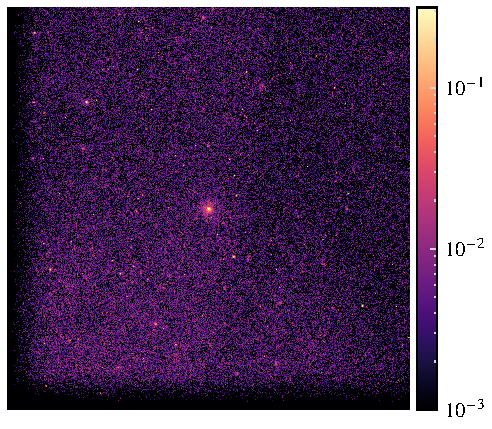
\includegraphics[width=\textwidth,height=\textwidth,keepaspectratio]{data_reduction/combined_tiles_0_raw_0.2-2.3keV.pdf}
        \caption{\SIrange{0.2}{2.3}{\kilo\electronvolt}}
        \label{fig:low_energy}
    \end{subfigure}
    \hfill
    \begin{subfigure}{0.325\textwidth}
        \centering
        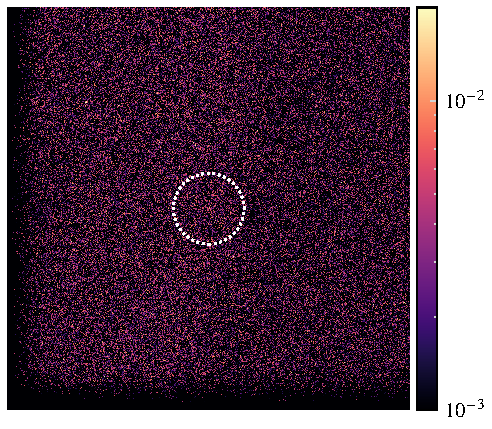
\includegraphics[width=\textwidth,height=\textwidth,keepaspectratio]{data_reduction/combined_tiles_0_raw_2.3-6.0keV.pdf}
        \caption{\SIrange{2.3}{6.0}{\kilo\electronvolt}}
        \label{fig:mid_energy}
    \end{subfigure}
    \hfill
    \begin{subfigure}{0.325\textwidth}
        \centering
        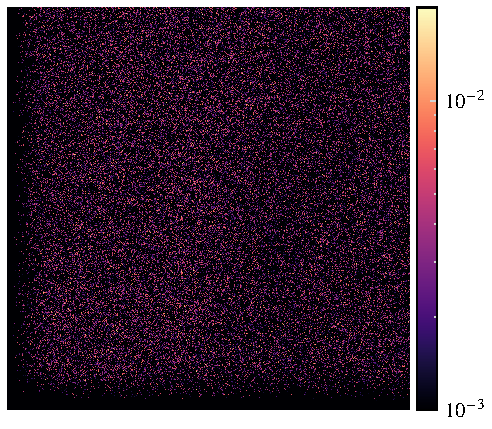
\includegraphics[width=\textwidth,height=\textwidth,keepaspectratio]{data_reduction/combined_tiles_0_raw_6.0-9.0keV.pdf}
        \caption{\SIrange{6.0}{9.0}{\kilo\electronvolt}}
        \label{fig:high_energy}
    \end{subfigure}
    \caption{Raw photon images from TM0 of all combined skytiles centered around NGC1550, displayed in the energy bands \SIrange{0.2}{2.3}{\kilo\electronvolt} (a), \SIrange{2.3}{6.0}{\kilo\electronvolt} (b), and \SIrange{6.0}{9.0}{\kilo\electronvolt} (c), with Gaussian smoothing of 4 pixels applied. The colorbar represents (smoothed) photon counts. For visualization purposes, different cuts were use for the middle and right image and \(R_{200}\) is shown (white dashed circle). Most of the group emission is visible in the lower energy band (\SIrange{0.2}{2.3}{\kilo\electronvolt}).}
    \label{fig:raw_photon_images}
\end{figure}
%
\section{Image filtering}
Each skytile is cleaned individually using \texttt{evtool} with \texttt{pattern=15} to select all event patterns and \texttt{flag=0xe00fff30} to remove bad pixels and CCD corners. Subsequently, soft proton flares are identified and mitigated through the following process: the \texttt{flaregti} task is used to generate light curves with \SI{20}{\second} time bins in the energy range of \SIrange{5}{10}{\kilo\electronvolt}. A \(3\sigma\) threshold is determined; time intervals where count rates exceed this threshold are likely due to soft proton flares. The task \texttt{flaregti} is then rerun using this threshold to establish good-time-intervals (GTIs) excluding these flare periods, which are applied using \texttt{evtool} with the \texttt{gti="FLAREGTI"} parameter. All SPF-filtered and cleaned skytiles are combined into a single TM0 photon image using \texttt{evtool}. Hereafter, these combined images shall be referred to as \enquote{filtered}.
%
\section{Exposure map and image creation}\label{sec:exposure_map}
The \texttt{evtool} task, along with the \texttt{telid} parameter, is used to split the TM0 filtered photon images into individual filtered images for each TM. These images are then resized to the soft-band and the hard-band using \texttt{evtool} with the parameters \texttt{emin} and \texttt{emax}. For subsequent PIB and exposure corrections, both vignetted and flat (non-vignetted) exposure maps are generated for each TM in the soft band using the \texttt{expmap} task with the \texttt{withvignetting} parameter. Moreover, the \texttt{withdetmaps} parameter is specified to crop the images at the edge of the field of view for each TM. By keeping \texttt{withmergedmaps} at its default value of \texttt{YES}, merged all-telescope exposure maps are created. This means the exposure maps consider the 7 TMs as one TM with on-chip TM, assuming the combined effective area of the 7 on-chip TMs. The vignetted and flat exposure maps can be found in Appendix TODO.
\section{PIB Correction}
It is necessary to subtract the particle-induced background (PIB) from the combined filtered photon image. The following  approach is based on extensive studies of the eROSITA filter wheel closed (FWC) data conducted by Dr. F. Pacaud, as utilized for example in \citep{Reiprich2021}.  The PIB is modeled for each TM using FWC data. Due to the minimal spatial variation of the PIB, this modeling utilizes the flat exposure map created in Section \ref{sec:exposure_map}. Furthermore, given the negligible spectral variation, the counts \(H_\text{obs}\) in the hard band, where PIB counts dominate, is used to estimate the PIB contribution in the soft bands by multiplication with the ratio \(R\) of the number of FWC counts in the soft band \(S_{\text{FWC}}\) to the hard band \(H_\text{FWC}\). The PIB-map for each TM is then generated by applying this factor to the flat exposure map, normalized to 1 by dividing by the sum of all pixel values (norm. flat exposure map). Hence, the PIB map of a given TM is given by
\begin{align*}
    \text{PIB map}_\text{TM} = H_\text{obs}R\cdot\bigl(\text{norm. flat exposure map}\bigr).
\end{align*}
Soft-band, PIB-corrected image are obtained by subtracting the PIB map of each TM from the respective soft-band, filtered photon image. The complete image for TM0 is obtained by co-adding all PIB corrected images. To better visualize the PIB-correction, individual background maps are also co-added to form a complete PIB map, which can be found in Appendix \ref{sec:appendix_a_pib_map}. Appendix \ref{appendix_a_pib_map} also contains the obtained \(H_\text{obs}\) and \(R\) values.
%
\section{Absorption Correction}
As discussed in Section \ref{sec:background}, X-ray absorption by the ISM must be considered. To correct for this absorption, the methodology outlined in \citep{Reiprich2021} is followed. Additionally, scripts for the absorption correction were provided by Angie Veronica (as utilized in \cite{veronica2020}). At energies \(\gtrsim \SI{0.2}{\kilo\electronvolt}\), as is relevant for this analysis, absorption from metals play a significant role (cf. \ref{sec:background}). 
Assuming solar metallicity, the hydrogen column density \({\textstyle (N_\text{H})}\) can be used to trace the absorbing material. A cutout of the HI4PI all-sky survey (\cite{HI4PI2016}) is reprojected onto field of view of the combined tile image to create a neutral atomic hydrogen map (\({\textstyle N_{\text{HI}}}\)-map). Additionally, as outlined in \citep{Willingale2013}, a molecular hydrogen map (\({\textstyle N_{\text{H}_2}}\)-map) is constructed by dividing the full sky image into \(52 \times 52\) pixel cells, querying \({\textstyle N_{\text{H}_2}}\) values from the Swift homepage\footnote{\url{https://www.swift.ac.uk/analysis/nhtot/index.php} (Last accessed: 25.07.2024)}, and distributing these values across each cell. The total \({\textstyle N_{\text{Htot}}}\)-map, constructed by \({\textstyle N_{\text{Htot}} = N_{\text{H}} + 2N_{\text{H}_2}}\), is shown in Figure \ref{sec:appendix_a_NH_corr}, with \({\textstyle N_{\text{H}}}\) ranging from \({\textstyle N_\text{Htot, min} = \SI{2.91e+20}{{\centi\meter}^{-2}}}\) to \({\textstyle N_\text{Htot, max} = \SI{1.61e+21}{{\centi\meter}^{-2}}}\).
Next, for a each individual \({\textstyle N_{\text{H}}}\)-value in the \({\textstyle N_{\text{Htot}}}\)-map, the expected soft band count rates for TM1 and TM5 -- which serve as proxies for TM8 and TM9, respectively -- are simulated for the model
\begin{align*}
    \text{apec}_{\text{LHB}} + \text{tb}_\text{abs.}\cdot(\text{apec}_{\text{MWH}} + \text{pow})
\end{align*}
using the X-ray spectral fitting package XSPEC\footnote{\url{https://heasarc.gsfc.nasa.gov/xanadu/xspec/} (Last accessed: 25.07.2024)} (\cite{Arnaud1996}) with the \texttt{fakeit} command and their respective area (ARF) and response files (RMF). Here, \(\text{apec}_{\text{LHB}}\) represents unabsorbed Local Hot Bubble emission, \(\text{tb}_\text{abs.}\) the absorption along the line of sight, \(\text{apec}_{\text{MWH}}\) the absorbed Milky Way Halo emission, and \(\text{pow}\) the absorbed emission from unresolved point sources (e.g., AGNs). A correction factor \(A_{\text{corr}}\) is determined for each value of \(N_\text{H}\) by dividing the simulated count rate for the \({\textstyle N_{\text{Htot}}}\)-map median \({\textstyle \bigl(\overline{N_{\text{Htot}}}\bigr)}\) by the simulated count rate of the \({\textstyle N_{\text{H}}}\) of interest, hence
\begin{align*}
    A_{\text{corr}}(N_\text{H}) = \frac{\text{simulated count rate}\bigl(\overline{N_{\text{Htot}}}\bigr)}{\text{simulated count rate}\bigl(N_\text{H}\bigr)}.
\end{align*}
Finally, each \(\textstyle{N_\text{H}}\) in the \({\textstyle N_\text{Htot}}\)-map is replaced by the corresponding correction factor \(A_\text{corr}\) to create an absorption correction map. Absorption correction maps are created for both TM1 and TM5.
%
\begin{figure}[htbp]
    \centering
    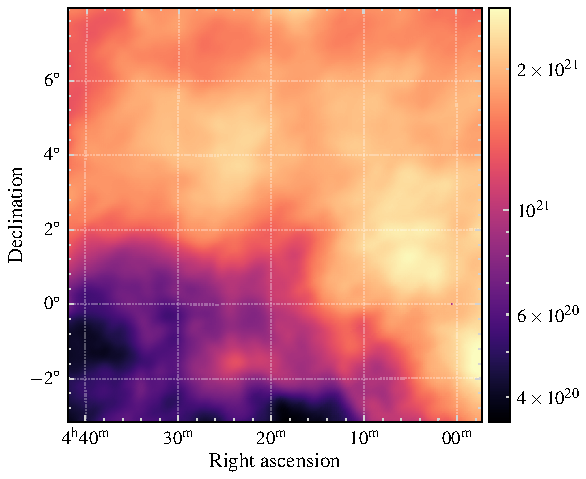
\includegraphics{appendix_a/NH_map.pdf}
    \caption{\(N_{\text{H}}\)-map}
    \label{fig:pib_map}
\end{figure}
%
\section{Exposure Correction}\label{sec:exposure}
The count image of any given X-ray observation depends inherently on a detector's effective area and the telescope's pointing motion throughout the observation. To obtain meaningful flux units (e.g. \(\text{cts}\cdot\text{arcsecond}^{-2}\text{s}^{-1}\)), these effects must be considered. This is achieved by dividing the count image by the vignetted exposure map created in Section \ref{sec:exposure_map}, thereby rescaling all segments of the count image to the same relative exposure (\cite{davis2001formal}). However, an exposure map must be created separately for TM8 and TM9 due to three reasons: first, TM9 uses a narrower energy band, which lowers its expected count rate; second, this narrower energy band necessitates a different absorption correction map; third, TM8 and TM9 have very distinct area response files because of their different filter configurations. Thus, both exposure maps cannot simply be combined but must be corrected for these effects. The procedure outlined in \citep{Reiprich2021} will be followed. First, the vignetted exposure map of TM8 and TM9 are divided by their respective absorption correction maps to obtain an absorption-corrected exposure map (\(\text{exmap}_\text{TM8, corr}\), \(\text{exmap}_\text{TM9, corr}\)). Second, the ratio of PIB-corrected count rates of TM8 and TM9 is used to define a correction factor 
\begin{align*}
    E_\text{corr} = \frac{\text{PIB corr. count rate(TM9)}}{\text{PIB corr. count rate(TM8)}}.
\end{align*}
The total absorption-corrected exposure map for TM0 is then given by
\begin{align*}
    \text{exmap}_\text{TM0, corr} = \text{exmap}_\text{TM8, corr} + E_\text{corr}\cdot\text{exmap}_\text{TM9, corr} 
\end{align*}
A correction factor of \(E_\text{corr} = 0.4628\) is obtained. Dividing the filtered and PIB-corrected soft-band TM0 image by its absorption-corrected exposure map results in the final filtered, PIB-corrected, absorption-corrected, and exposure-corrected soft-band image. Henceforth, this will be referred to as the \enquote{corrected} soft-band image. Figure \ref{fig:comparison_filt_corr} compares the filtered, full energy-band count rate image (the filtered full band count image divided by its respective exposure map) with the corrected soft-band image, both smoothed using a Gaussian kernel of 12 pixels. It is evident that group emission can be much better distinguished from the background in the corrected soft-band image. Additionally, it was noted in Section \ref{sec:raw_photon} in Figure \ref{fig:raw_photon_images}, has been addressed through the absorption and exposure correction.
\begin{figure}[htbp]
    \centering
    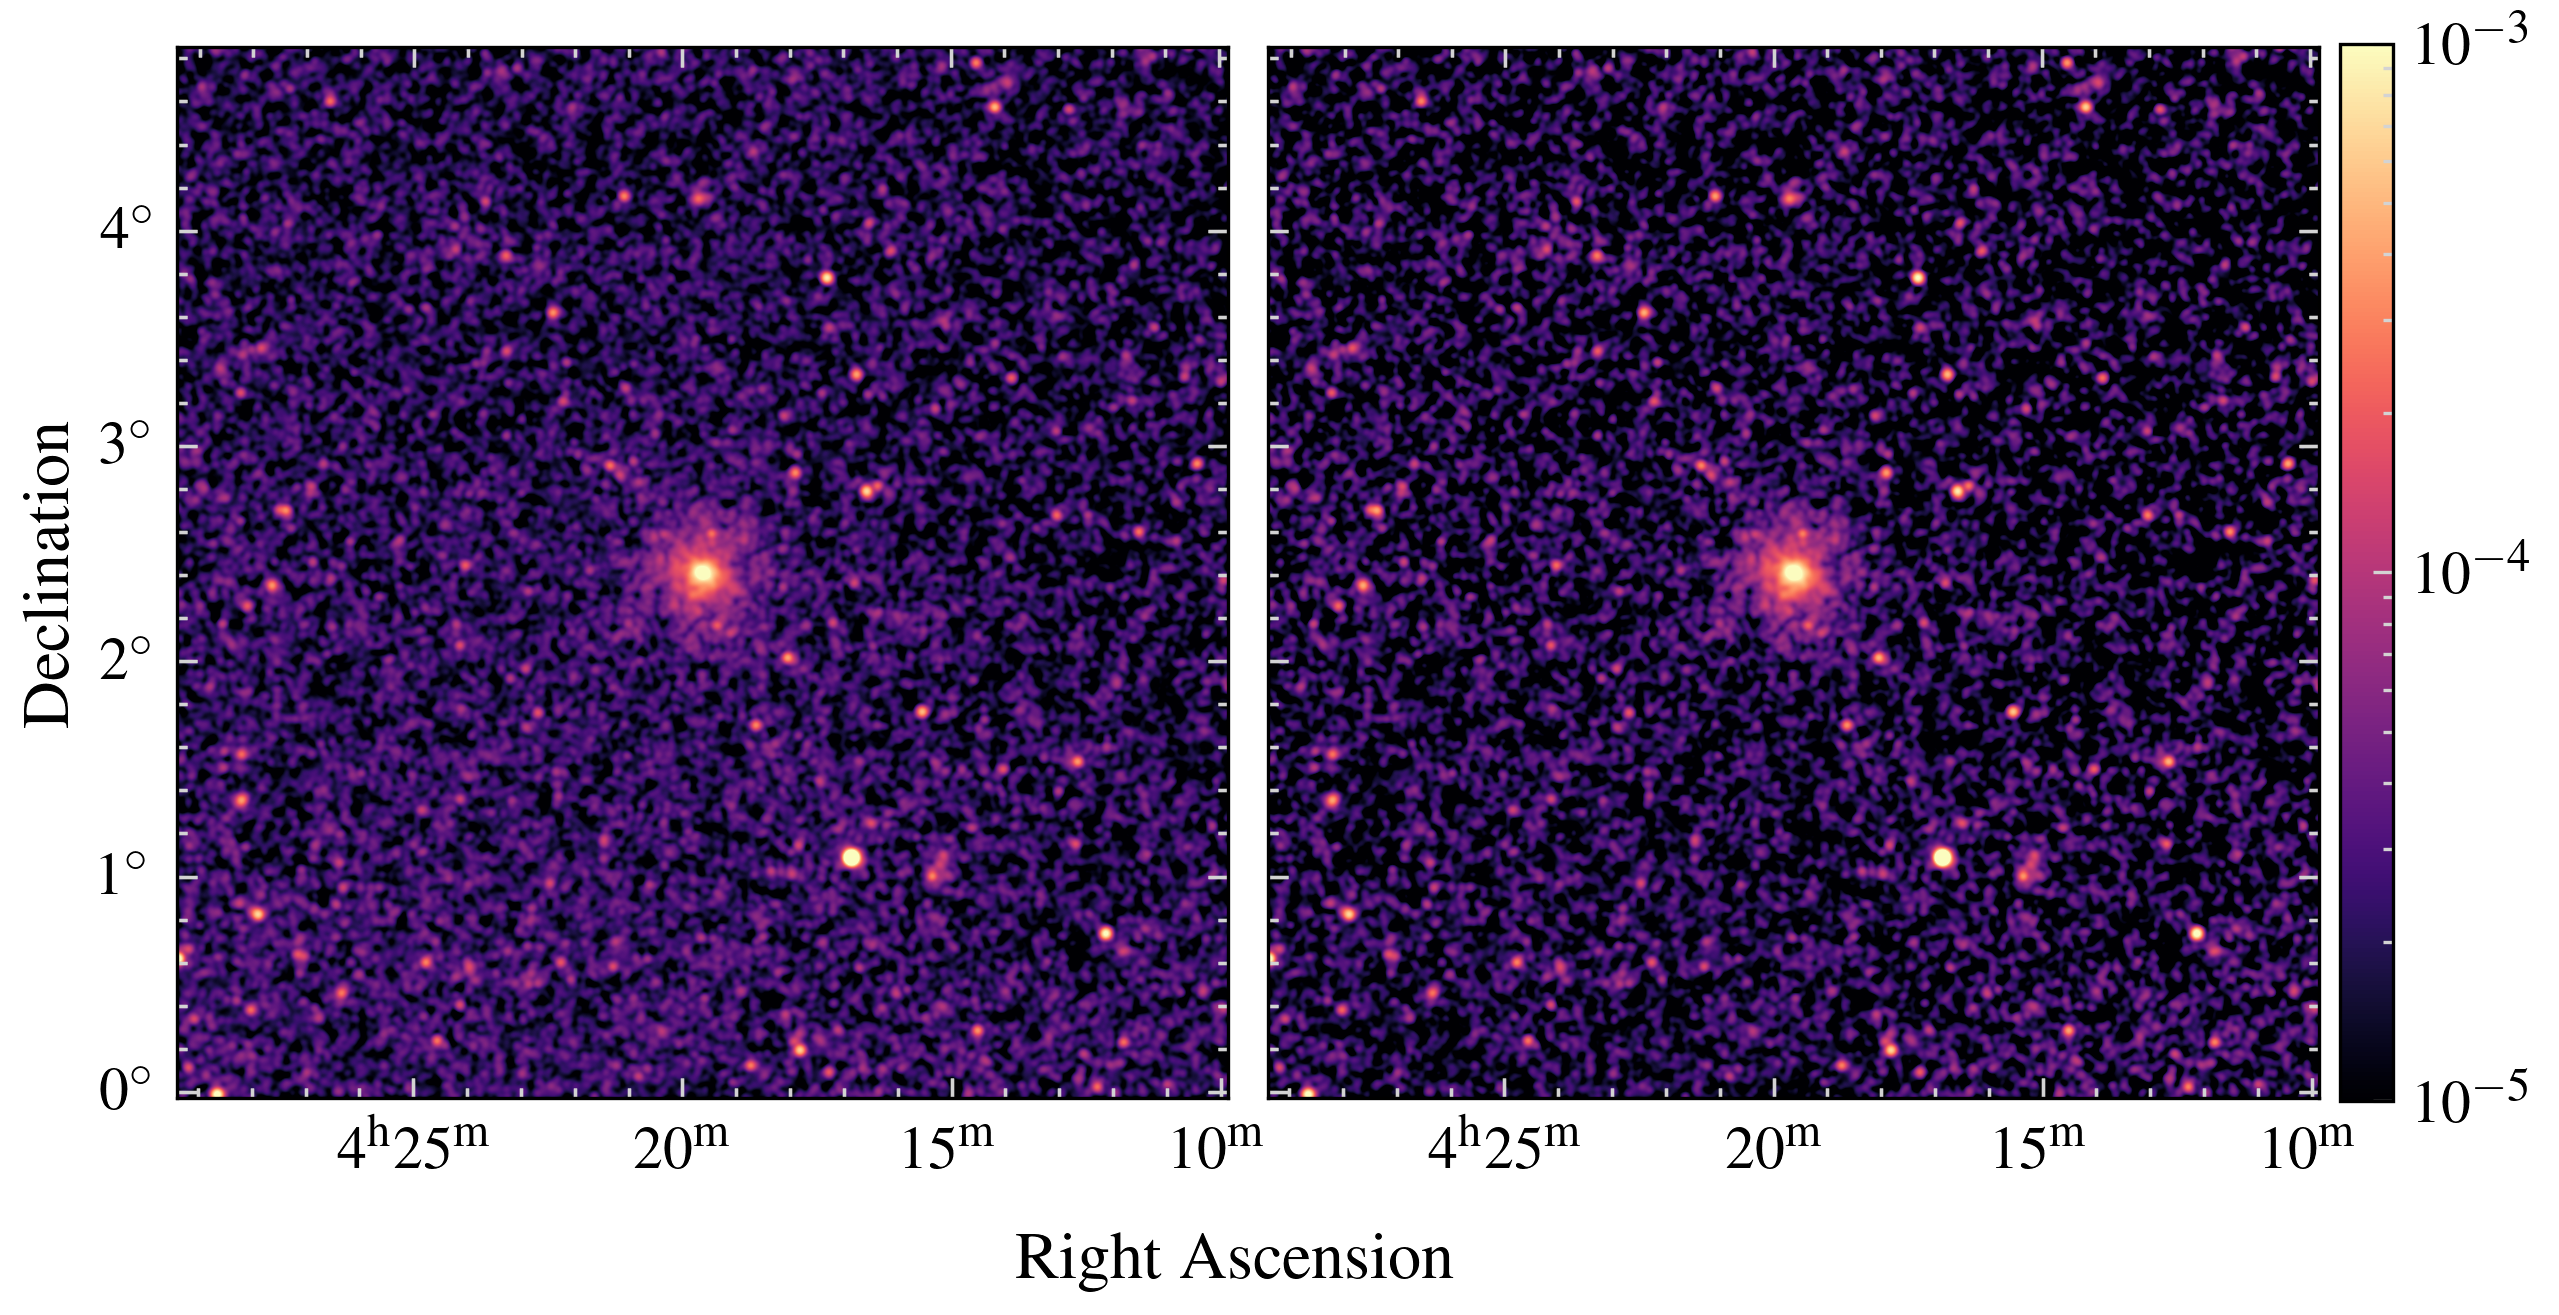
\includegraphics{data_reduction/filtered_corr_comparison.png}
    \caption{Comparison between the filtered, full energy-band count rate image (left) and the final corrected count rate image (right), both smoothed using a Gaussian kernel of 12 pixels. The corrected image clearly shows improved differentiation of group emission from the background in comparison to the filtered, full band image.}
    \label{fig:comparison_filt_corr}
\end{figure}
\section{Wavelet filtering and Point Source Removal}
It is necessary to remove the emission from point-like (e.g. AGNs) and unrelated extended sources to prevent interference with the group emission under study. This is achieved using the wavelet filtering pipeline as described in \citep{Pacaud2006}. Wavelet transformation decomposes an image \(I(x, y)\) into coefficients \((w_1, \ldots, w_n, c_n)\)
\begin{align*}
I(x, y) = c_n(x, y) + \sum_{j=1}^{n}w_j(x, y).    
\end{align*}
Here, \(c_n(x, y)\) is the smoothed image, and \(w_j(x, y)\) essentially represents the contribution of a wavelet function at a scale \(j\) and position \((x, y)\) to the total image. By retaining only the coefficients that satisfy
\begin{align*}
|w_j(x, y)| > k\sigma_j,
\end{align*}
where \(\sigma_j\) is the standard deviation at scale \(j\) and \(k\) is a clipping factor, and then applying the inverse wavelet transformation, an image is obtained that includes only significant scales, i.e. those not due to noise (\cite{Stark1998}). The resultant image is referred to as a wavelet-filtered image. In the pipeline being used, the absorption-corrected exposure map, \(\text{exmap}_\text{TM0, corr}\), and the filtered photon image are used to account for previous data reduction and to statistically handle the Poisson noise. After wavelet filtering, a source catalogue is obtained by \texttt{SExtractor} (\cite{Bertin1996}). This is enabled by the significant noise reduction and smoothed background achieved by the wavelet filtering. The extended X-ray emission near NGC1550 is manually removed from the catalog, and a cheese-mask is created from the catalog and applied to \(\text{exmap}_\text{TM0, corr}\). Emission around unrelated, but projectionally nearby, clusters and groups is also manually added to the cheese-mask. Rerunning wavelet filtering with the cheese-masked map reduces ringing artifacts, which typically occur near bright sources with steep flux gradients. Figure \ref{fig:comparison_wvl_filtered} compares the wavelet filtering before and after application of the cheese-mask to the exposure map.
%
\begin{figure}[htbp]
    \centering
    \begin{subfigure}[b]{0.48\textwidth}
        \centering
        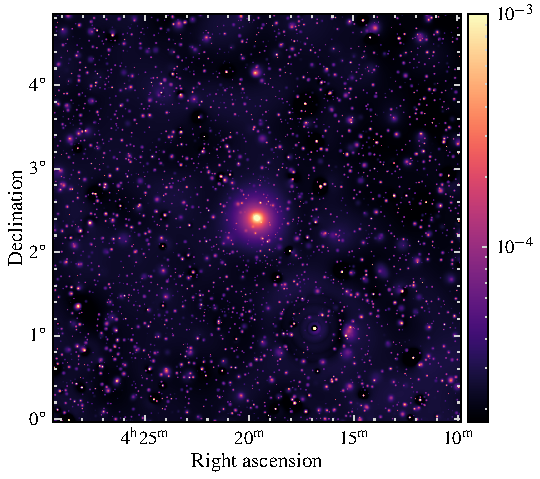
\includegraphics[width=\textwidth]{data_reduction/wlt_filtered.pdf}
        \caption{Before applying the cheese-mask}
        \label{fig:wlt_filtered}
    \end{subfigure}
    \hfill
    \begin{subfigure}[b]{0.48\textwidth}
        \centering
        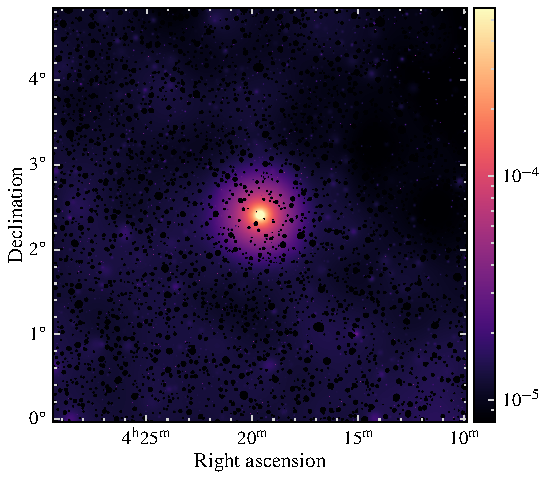
\includegraphics[width=\textwidth]{data_reduction/wlt_filtered_cheese.pdf}
        \caption{After applying the cheese-mask}
        \label{fig:wvl_filtered_cheesed}
    \end{subfigure}
    \caption{Corrected wavelet filtered image before (a) and after (b) applying the cheesemask created with \texttt{SExtractor}. The left image is normalized such that the ringing artifacts are more prominent. The cheese-masked image has significantly reduced ringing artifact and group emission is well visible.}
    \label{fig:comparison_wvl_filtered}
\end{figure}




